\documentclass{report}   %Documento tipo reporte
\usepackage[spanish]{babel}    %Paquete de Idioma
\usepackage{float, graphicx, caption, color, amsmath}
\usepackage[hidelinks]{hyperref}

\begin{document}


\begin{titlepage}    %Portada
	\centering
	{\huge\bfseries Proyecto de investigación: \par}
	\vspace{1cm}
	{\huge\bfseries  Interrupciones \par}
    \vspace{3cm}
    {\scshape\large Valentina Botero Vivas \par}
    \vspace{3cm}
      {\scshape\large Docente  \par}
	\vspace{0.5cm}
    {\scshape\large Augusto Salazar Jimenez  \par}
	\vspace{3cm}
	 {\scshape\large Universidad de Antioquia \par}
	\vspace{1cm}
    {\scshape\large Informática II  \par}
	\vspace{1cm}
	{\large 3 de Julio del 2020 \par}
\end{titlepage}


Las interrupciones son recursos o mecanismos del microcontrolador para responder a eventos,permitiendo suspender temporalemnte el programa principal, para ejecutar una subrutinaUna, una vez la subrutina esté terminada, se reanuda la ejucución del program principal..\\

Entonces, la interrupción viene determinada por la ocurrencia de una señal, la cual provoca un desvío a una dirección específica de memoria, esto interrumpe momentánamente la ejecución del programa . A partir de esta dirección se encuentra la rutina de tratamiento que se encarga de realizar la subrutina,devolviendo después el control al punto interrumpido del programa. Este proceso se ilustra en la figura \ref{fig:Interrupción}

\begin{figure}[H]
      \centering
      \captionsetup{justification=centering}
      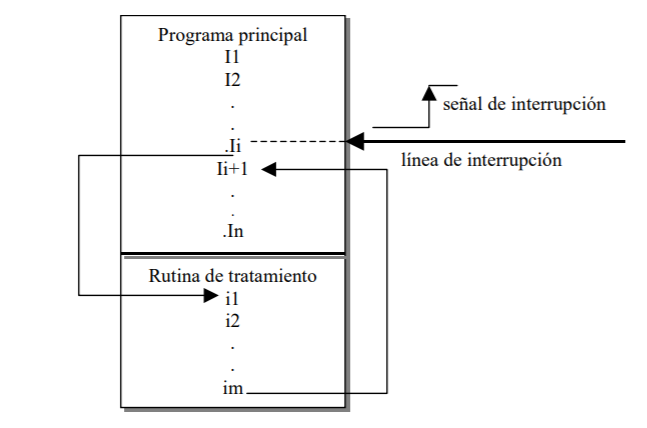
\includegraphics[scale=0.7]{1.PNG}
      \caption{Interrupción ocasionada por señal externa. Tomado de \cite{3}}
      \label{fig:Interrupción}
   \end{figure}

Las interrupciones son de gran importancia ya que aumentan el rendimiento de los sistemas. 

\section*{Historia}
Si se busca hablar de la historia de las interrupciones, es importante aclarar que éstas fueron necesarias y aparecieron como solución a un problema.\\\\
Surgen de las necesidades que tienen los dispositivos periféricos de enviar información al procesador principal de un sistema de computación.\\\\ Por ejemplo, en los primeros sistemas cuando una aplicación necesitaba leer la pulsación de una tecla, interrogaba continuamente al teclado, es decir, sondeaba el dispositivo cada cierto tiempo hasta que la tecla fuera presionada, teniendo en cuenta que mientras se esperaba una tecla, no se podían ejecutar otras tareas.\\ La solución a este problema apareció con la llamada interrupción de teclado en donde el controlador del dispositivo, en este caso el teclado, es quien genera una interrupción sólo cuando el dispositivo está listo para transferir datos.\\ En este caso, el microprocesador, no sondeaa ningún dispositivo, sino que queda a la espera de que estos le avisen (le "interrumpan") cuando deba ejecutar una subtarea.

En los microcontroladores se emplea un dispositivo denominado controlador de interrupciones o unidad de interrupciones que tiene como función controlar la solicitud de eventos o dispositivos periféricos.

\section*{Tipos de interrupciones}
Las interrupciones pueden ser:
\begin{itemize}
\item Síncrónicas:  Generadas por el sistema al ejecutar instrucciones.
\item Asincrónicas: Generadas por otros dispositivos no están alineadas con el reloj del sistema.
\end{itemize}

Debido a la fuente que los produce, pueden clasificarse en tres tipos:

\section*{Interrupciones de hardware}
Estas interrupciones son asincronas, es decir se pueden producir en cualquier momento sin importar lo que este haciendo el sistema. No son producidas por ninguna instrucción de un programa sino por las señales que emiten los dispositivos periféricos para indicarle al procesador que necesitan ser atendidos.

\begin{itemize}
    \item Internas: Generadas por eventos durante la ejecución de alguna tarea. Son manejadas en su totalidad por hardware y no es posible modificarlas.
    \item Externas: Generadas por los dispositivos periféricos.No es posible desactivarlas. Existen dos tipos:
      \begin{itemize}
        \item{Enmascarables:}
        El procesador no puede atenderla o la ignora.Se usan para la atención del periférico.
        \item{No enmascarables:}
        El procesador no puede evitar atenderlas y tienen mayor prioridad.
  \end{itemize}
  
  Estas interrupciones son señales generadas desde dispositivos físicos. Así le informan al procesador que el dispositivo requiere atención, ahí es cuando se detiene la ejecucuión principal. Pueden originadas desde dispositivos como teclados, reloj,impresora,puerto serie, etcétera.
\end{itemize}
\section*{Interrupciones de software}
Estas interrupciones son sincronas, ya que se producen cuando un usuario solicita un llamado al sistema. Es dcir, son generadas por un programa mientras se está ejutando. Este tipo de interrupciones se pueden separar en dos tipos:
\begin{itemize}
        \item{Iterrupciones del sistema operativo.}
        \item{Interrupciones del usuario:} 
  \end{itemize}
  
El sistema operativo es un sistema de control y como tal controla la ejecución de los programas. Las interrupciones por software dependen de las llamadas al sistema y estas no dependen de los lenguajes de programación,ni del hardware, ya que la interrupción solo es una petición o llamado al sistema operativo.

\section*{Excepciones}
Estas son sincrónicas, se dan cuando se detecta una situación de error mientras se ejecutaba una instrucción.
Su principal diferencia es que mientras que en las interrupciones el programa principal se pone en pausa, en las excepciones la istrucción a bordo es abortada.
\section*{Orden de prioridad:}
\begin{enumerate}
    \item Excepciones.
    \item Interrupciones de software.
    \item Iterrupciones de hardware.
\end{enumerate}
Ahora en los microprocesadores hay dos tipos de interrupciones,la primera corresponde a eventos que generan un estado lógico (Cambio de voltaje). El segundo tipo corresponde a las interrupciones que pueden ser cambiadaspor softwareen los pines del microprocesador.\\\\


El ejemplo práctico realizado con arduino se ve en el video adjunto, se desarrolló siguiendo los pasos de \cite{6}

\begin{thebibliography}{0}
  \bibitem {1}Concepto de interrupciones. (s.f) .Lenguaje ensamblador.
  https://leo-yac.wixsite.com/lenguaje-ensamblador/el-concepto-de-interrupciones
  \bibitem{2} Jorge Luis Tinoco.(2011). Interrupciones del microprocesador. https://es.slideshare.net/jorg-leoxd/interrupciones-del-microprocesador
  \bibitem{3} Interrupciones.(s.f). Estructura de computadores,Facultad de Informática,UCM. http://www.fdi.ucm.es/profesor/jjruz/WEB2/Temas/Curso05-06/EC9.pdf
  \bibitem{4}Kishin Aimura.(2014).Interrupciones y excepciones del S.O.https://prezi.com/k-shlyu6hqr2/interrupciones-y-excepciones-del-so/\bibitem{5} Iterrupciones de entrada y salida.(2012).http://mariolopezchavez.blogspot.com/
  \bibitem{6} Luis del Valle Hernández.(s.f).Interrupciones con Arduino a través de un ejemplo práctico. https://programarfacil.com/blog/arduino-blog/interrupciones-con-arduino-ejemplo-practico/
\end{thebibliography}

\end{document}
